\chapter{AlterNative}\label{C:AlterNative}
This chapter is a walk-through AlterNative explaining its concept, how translates the code, then an example using IOSharp will be used along with some use cases that can be applied to this tool.
\section{Concept}\label{S:AN-Concept}
The concept of AlterNative is to maximize the idea of Internet of Things by providing a tool to port applications from high-level languages (such as .NET) to native languages (such as C++) easily. Most of the actual systems are C++ compatible, thus if the application is ported to this language, it can be executed in several platforms (i.e. smartphones, tablets, embedded systems, computers with different operating systems).
\\
With this tool a developer can take the advantages of fast developing in a high-level languages such as C\# and then gain the advantage of performance related the low-level languages like C++. Apart from this it also gives the possibility to get native code capable of work in several systems, in other words, this philosophy is similar to the WORA (Write Once, Run Anywhere) slogan created by Sun Microsystems to illustrate the cross-platform benefits of Java Virtual Machine. The difference is that AlterNative is focused on the final performance because it outputs the original code in native language and does not depend on any virtual machine.
\section{Process}\label{S:AN-Process}
AlterNative process is divided in three steps: decompilation, translation and recompilation.
To summarize the following sections the figure \ref{fig:AN-Process} shows the process that is done from the original assembly, the decompilation, translation and recompilation to a native assembly.
\begin{figure}[H]\begin{center}
 \centering
  \captionsetup{justification=centering}
  \includegraphics[width=1\textwidth]{pictures/alternative/process}
  \caption{AlterNative process\label{fig:AN-Process}}
\end{center}\end{figure}

\subsection{Decompilation}\label{SS:AN-Process-Decom}
First of all the Assembly (compiled program/binary) is passed through a decompiler in order to extract the source code. In this case the code extracted is C\# and to decompile it is used the ILSpy which is an open-source .NET assembly decompiler. The code is not extracted in text format, but in an AST (Abstract Syntax Tree) that is an abstract representation with nodes and hierarchies of the original code. This representation is organized in a tree from the top-level (Assembly) until de low-level (instructions, types and constants).
\\
\\
The figure \ref{fig:AN-AST} shows how the \verb!void Main(string[] args){}! method would look like in AST format. The top node designates that the child nodes correspond to a method, then in the first row child is described the primitive type (what would return the method) which is \verb!void! in this case, the identifier which shows the method name (\verb!Main!) and finally the parameter declaration which describes the parameters that the function takes. In the method shown in the example has one parameter corresponding to an array of strings. The parameter declaration node has two nodes defining it, the first one describes that \verb!string[]! is a composed type by a string and an array specifier, the second node is the identifier name of the parameter, in this case, \verb!args!.
\begin{figure}[H]\begin{center}
 \centering
  \captionsetup{justification=centering}
  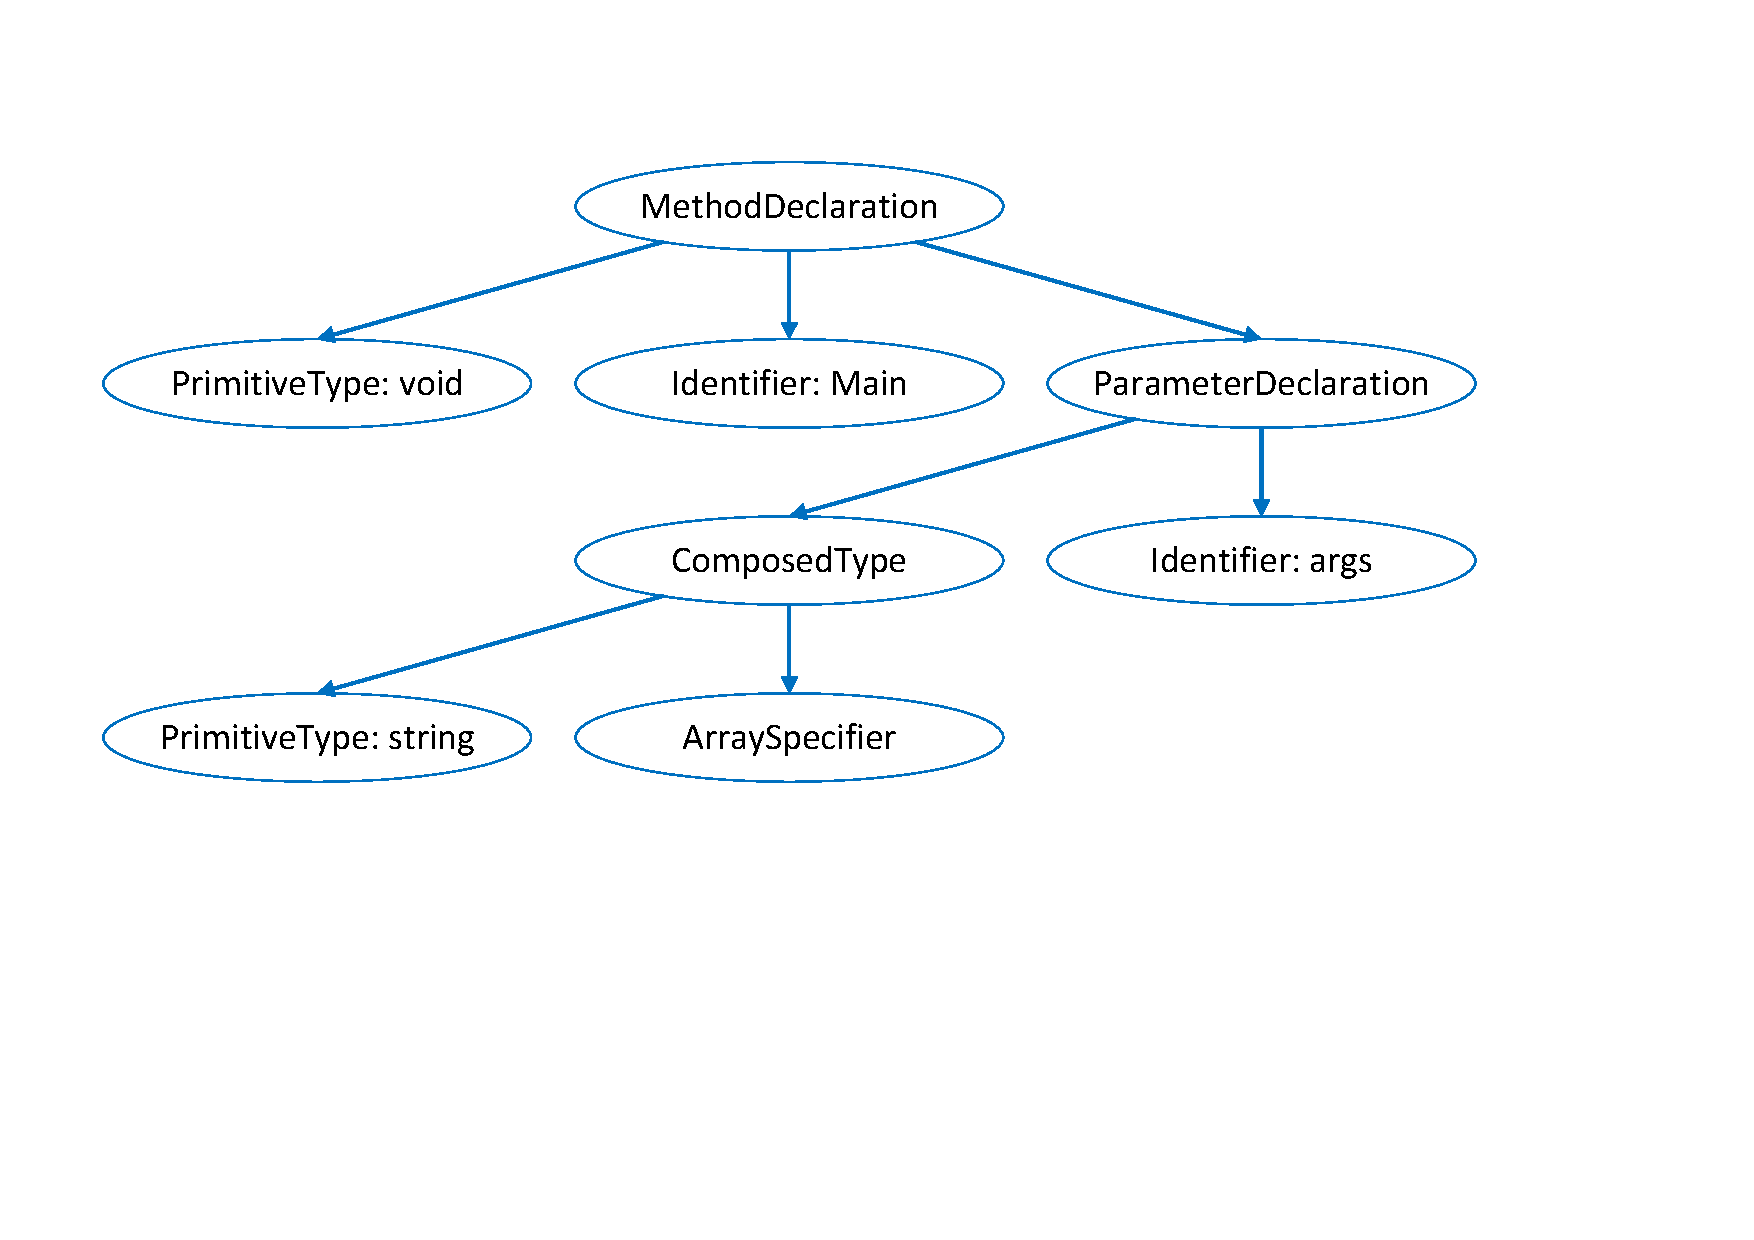
\includegraphics[width=0.7\textwidth]{pictures/alternative/csharp_main_ast}
  \caption{AST representation of the main method in C\#\label{fig:AN-AST}}
\end{center}\end{figure}
The translator will generate the C++ code from the AST representation of the original code.
\subsection{Translation}\label{SS:AN-Process-Translation}
To proceed with the translation it is important to know the how is typed the resulting language, then in order to achieve that some modifications need to be applied to the AST, by doing this a second AST will be obtained representing the source code of the desired language. After doing this conversions the following step is start writing the files containing the text representation of the tree. AlterNative translates the code to C++ so the AST changes must be done in a way that the resulting AST corresponds to that language. When printing the new code the headers and the code files must be printed.
\\
\\
Following the example explained in the previous section now the AST will be transformed to the correspond with the C++ one. In C\# the method was \verb!void Main(string[] args){}! but in C++ the syntax is different because the array specifier moves from the primitive type to the identifier. The figure \ref{fig:AN-AST-Conversions} shows in red the changes done to the original tree to achieve an AST corresponding to the C++ method which looks like \verb!void Main(string args[])!. The original identifier changes to a composed identifier with two child nodes, the first one is the identifier \verb!args! and the second one is the array specifier moved from the original composed type to the composed identifier. As there is no composed type now the node is deleted and the parameter declaration is directly linked to the primitive type string.
\begin{figure}[H]\begin{center}
 \centering
  \captionsetup{justification=centering}
  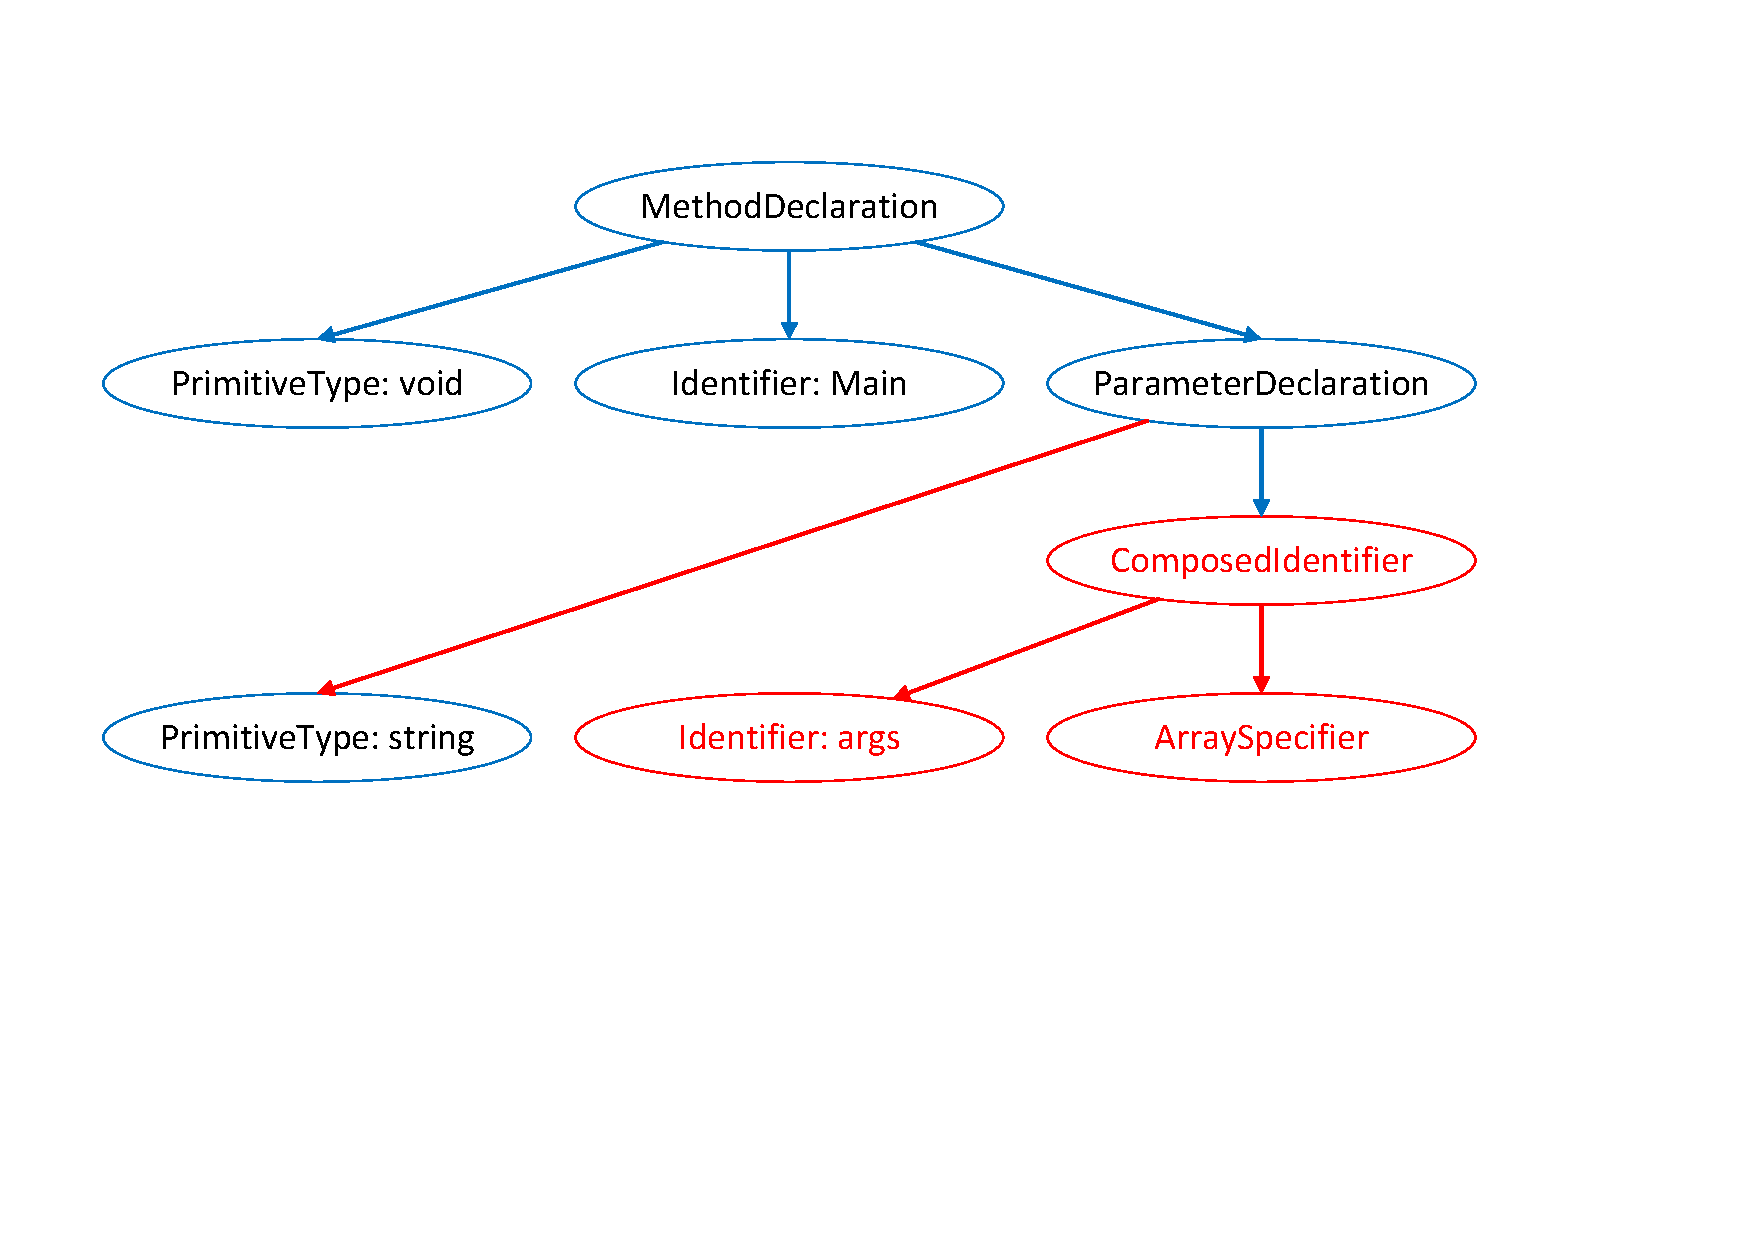
\includegraphics[width=0.7\textwidth]{pictures/alternative/ast_conversions_cpp}
  \caption{AST representation of the main method in C++\label{fig:AN-AST-Conversions}}
\end{center}\end{figure}

\subsection{Recompilation}\label{SS:AN-Process-Recompilation}
The final step consists on compile the C++ code into a new assembly. This final assembly maintains the same functionalities of the first one but taking the benefits of the performance that gives native code. Although it could seem that this software is focused on the code translation but it is not its real finality because its aim is to maintain all the features of the original code like the garbage collector, specific expressions or even language syntax. With all of this passed through AlterNative the program will run much faster than the original one because it is running in native code.
\\
AlterNative is able to provide most of the features of the original code to the final code using external open-source libraries like the boehm GC for the garbage collector, the boost library for the threading and datetime library and finally a proprietary library which implements all the \verb!System! namespace of C\#. With all of this the final assembly is fully compatible with any system like Windows, Linux, Android or any device capable of execute C++ binaries.

\section{Use Cases}\label{S:AN-Use-Cases}
There are two clearly use cases of AlterNative together with IOSharp, the first one is performance and the second one is generate cross-platform programs for embedded systems.
\subsection{Performance}\label{SS:AN-Use-Cases-Perf}
AlterNative gets the major advantage when is applied to programs or libraries which are very complex in a computational way for example image processing, mathematics or complex algorithms where languages running on virtual machines are not as fast as the developer needs. The more complex is the target, the more benefit that can be obtained.
Taking into account that the performance seen on IOSharp over Mono is not as good as it should be compared to the native Micro Framework with a Netduino. Is supposed that passing a program created with IOSharp (which runs on top of Mono) through the translator will generate a faster binary because it does not depend on a virtual machine , and is well known that Mono is not the fastest implementation of the .NET specification.

\subsection{Cross-Platform in embedded systems}\label{SS:AN-Use-Cases-NETMF}
Other advantage of the standard low level languages like C++ is that a high percentage of device processors can execute this code. And at this point is where fits with the implementation of IOSharp because passing the library through AlterNative a new library will be obtained but instead of being written in C\# it will be in C++. By doing this the generated source can be compiled into an ARM-Linux assembly so the unique requirement to execute that code will be an underlying Linux running on the machine. The developer will get all the benefits of Micro Framework with the speed of C++, the code will be written using IOSharp or native Micro Framework which is really easy to develop embedded applications with this software and then translate the program with AlterNative.

\section{Work done in AlterNative}\label{AN-WorkDone}
To achieve the translation (or partial translation) of IOSharp through AlterNative some work was done on the proprietary implementation of \verb!System! libraries which are the the C++ libraries that externally look like the C\# ones but the methods are implemented using standard C++ functions with the boost library or other libraries like the Boehm GC.
\\
\\
At the beginning AlterNative only worked on Windows because some classes from the ILSpy had mixed some functions for the view and some functions from the decompiler so it was unable to run in Linux because the part of the view could not compile. In order to solve that an AlterNative.Core was created which could work in any system that could run C\# code. This core version has its own solution and csproj file but they are pointed to the same code files of the original program. In this way AlterNative can run either on .NET Framework in Windows or on Mono in Linux and MacOSX.
\\
\\
The first attempt to translate IOSharp was unsuccessful but it helped to determine how much the translation was near to be successful. There where several major features that AlterNative was not able to translate like the threading, the delegates used in the interruptions, the P/Invokes or some functions like DateTime, Timer and file access to read and write. Many of these features need to be implemented on the proprietary library because this is linked to the translated program as C\# does with its own libraries.
\\
To implement this features the C++ boost library has been used. This library uses standard C++ functions so it can work in any device or operating system capable of execute binaries compiled from C++.

\section{Example}\label{SS:AN-Process-Example}
The best example to show in this section will be some of the parts of IOSharp translated to C++. In the moment of writing this thesis the only component working well in the translation was the GPIO ports which basically they use the \gls{SYSFS} of Linux and the interrupt port which uses calls to C is also working.
\\
\\
dfdf
\\
\\
Some performance tests had been carried out to quantify how much is faster the translation of IOSharp compared with the original one running on Mono. The explanation of the tests and its results are on the next chapter.